\documentclass[a4paper,11pt]{article}
\input{/home/tof/Documents/Cozy/latex-include/preambule_doc.tex}
\input{/home/tof/Documents/Cozy/latex-include/preambule_commun.tex}
\newcommand{\showprof}{show them}  % comment this line if you don't want to see todo environment
\setlength{\fboxrule}{0.8pt}
\fancyhead[L]{\fbox{\Large{\textbf{BAC 02}}}}
\fancyhead[C]{\textbf{Épreuves pratiques}}
\newdate{madate}{10}{09}{2020}
%\fancyhead[R]{\displaydate{madate}} %\today
\fancyhead[R]{Terminale - NSI}
\fancyfoot[L]{\vspace{1mm}Christophe Viroulaud}
\AtEndDocument{\label{lastpage}}
\fancyfoot[C]{\textbf{Page \thepage/\pageref{lastpage}}}
\fancyfoot[R]{\includegraphics[width=2cm,align=t]{/home/tof/Documents/Cozy/latex-include/cc.png}}

\begin{document}
\begin{exo}
    \begin{enumerate}
        \item Écrire une fonction \texttt{\textbf{recherche}} qui prend en paramètre un tableau de nombres entiers
              \texttt{\textbf{tab}}, et qui renvoie la liste (éventuellement vide) des couples d'entiers consécutifs
              successifs qu'il peut y avoir dans \texttt{\textbf{tab}}.
        \item Proposer un jeu de tests permettant de vérifier plusieurs cas de figures.
    \end{enumerate}
\end{exo}
\begin{exo}
    \begin{itemize}
        \item On appelle « mot » une chaîne de caractères composée avec des caractères choisis
              parmi les 26 lettres minuscules ou majuscules de l'alphabet.
        \item On appelle « phrase » une chaîne de caractères :
              composée avec un ou plusieurs « mots » séparés entre eux par un seul
              caractère espace ' ', se finissant :
              \begin{itemize}
                  \item soit par un point '.' qui est alors collé au dernier mot,
                  \item soit par un point d'exclamation '!' ou d'interrogation '?' qui est alors séparé du dernier mot par un seul caractère espace ' '.
              \end{itemize}
    \end{itemize}
    \begin{enumerate}
        \item Construire plusieurs exemples de phrase et observer le lien entre le nombre d'espaces et le nombre de mots.
        \item Écrire la fonction \textbf{\texttt{nombre\_de\_mots(phrase: str) $\rightarrow$ int}} qui renvoie le nombre de mots dans \textbf{\texttt{phrase}}.
    \end{enumerate}
\end{exo}
\begin{exo}
    Un arbre binaire de caractères est stocké sous la forme d’un dictionnaire où les clefs sont les caractères des nœuds de l’arbre et les valeurs, pour
    chaque clef, la liste des caractères des fils gauche et droit du nœud.
    \begin{center}
        \centering
        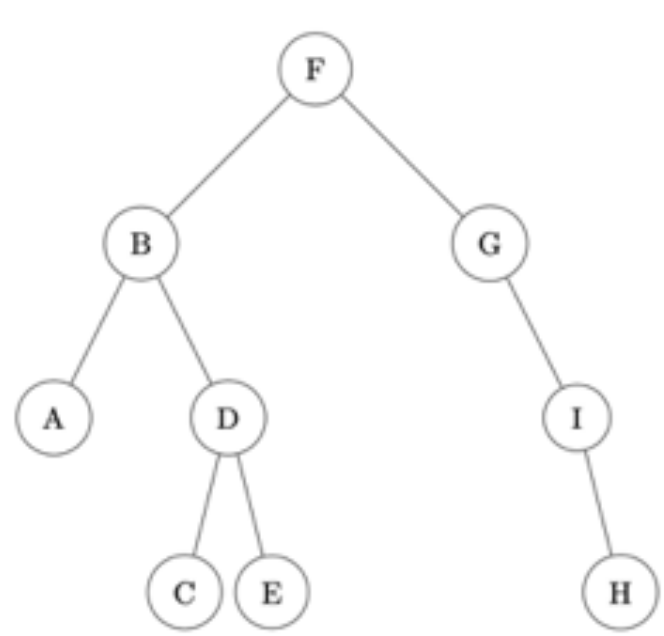
\includegraphics[width=8cm]{ressources/arbre.png}
    \end{center}
    \begin{enumerate}
        \item Construire le dictionnaire \textbf{\texttt{arbre}} représentant l'arbre binaire ci-dessus.
        \item Écrire la fonction récursive \textbf{\texttt{taille(arbre: dict) $\rightarrow$ int}} qui renvoie la taille de l'\texttt{\textbf{arbre}}. 
    \end{enumerate}
\end{exo}
\end{document}